\chapter{Dialog}

Conform definiției din limba română, dialogul este modul de expunere care prezintă succesiunea replicilor dintr-o conversație care are loc între două sau mai multe persoane.

Această lucrare își propune să dea formă înțelegerii limbajului natural dintr-o perspectivă matematică, prezentând sub forma unei soluții programabile un întreg sistem de micro servicii toate funcționând sub umbrela aceluiași scop, comunicarea.

Pe parcursul lucrării se va face referire la dialog ca o secvență de replici între un om și un calculator pentru a transmite informații.
Referitor la componentele unui dialog, se va prezenta doar o abordare bazată pe componenta \textit{verbală}, celelalte componente - \textit{nonverbală} (gesturi, mimică, poziția corpului) și \textit{paraverbală} (accentul, ritmul și intensitatea vorbirii) - făcând obiectul altor lucrări viitoare.


\section{Conversația naturală}

Un factor cheie într-o conversație este acela că fiecare replică dintr-un dialog este o formă de \textbf{acțiune} venită din partea vorbitorului \cite{witt1953}. În literatura de specialitate \textbf{actele de vorbire} sunt cele ce dau tipul acestor acțiuni.

De-a lungul timpului s-au propus numeroase moduri de a grupa acte de vorbire, iar modul de clasificare potrivit abordării de față conține doar 4 categorii și se concentrează pe intenția comunicată, conținutul propozițional și contextul de producere.

\subsection{Acte de vorbire}
\begin{enumerate}
	\item \textbf{Reprezentative (asertive)} - sunt acele acte care definesc o constatare. Cu ajutorul lor se comunică informații se impun constrângeri, iar la nivel de conținut putem spune că descriu realitatea. Se descriu anumite evenimente ("Coletul a fost livrat"), sau se impun anumite constrângeri ("Voi pleca maine"). Mărcile acestui act de vorbire sunt date de verbe precum: \textit{a afirma, a admite, a anunța, a avertiza, a declara, a insista, a înștiința, a zice, etc}.

	\item \textbf{Directive} - sunt actele ce urmăresc impunerea unei acțiuni. Scopul lor este de a determina participanții la dialog să execute o sarcină. Verbele marcante sunt \textit{a întreba, a interzice, a ordona, a cere}
	
	\item \textbf{Expresive} -  reprezintă o manifestare în plan verbal a sentimentelor, emoțiilor și a atitudinilor vorbitorului cu referire la acțunile întreprinse sau nu de către interlocutor. Verbele reprezentative ale acestui act sunt: \textit{a mulțumi, a lăuda, a felicita, a regreta, a reproșa, a critica, a acuza, etc}
	
	\item \textbf{Comisive (promisive)} - vizează angajamentul locutorului de a da curs unor acțiuni/convingeri \textit{a promite, a plănui, a jura, a paria, a se opune}
\end{enumerate}

Pentru stabilirea intenției, actul de vorbire joacă un rol foarte important, iar sistemele de dialog extind aceste clasificări în intenții specifice domeniului cu scopul de a caracteriza cât mai bine conversația.

%todo: Exemplu de intenții si cum sunt ele văzute in administratorul de dialog.

\section{Sistem de dialog}
Conversația cu un robot presupune o înlănțuire de servicii văzută ca un ciclu de informații ce se mulează pe intențiile vorbitorului. În continuare sunt prezentate componente care fac posibilă această conexiune.
% todo: de descris fiecare modl ]n parte
\subsection{Componente}
\begin{figure}[h]
	\centering
	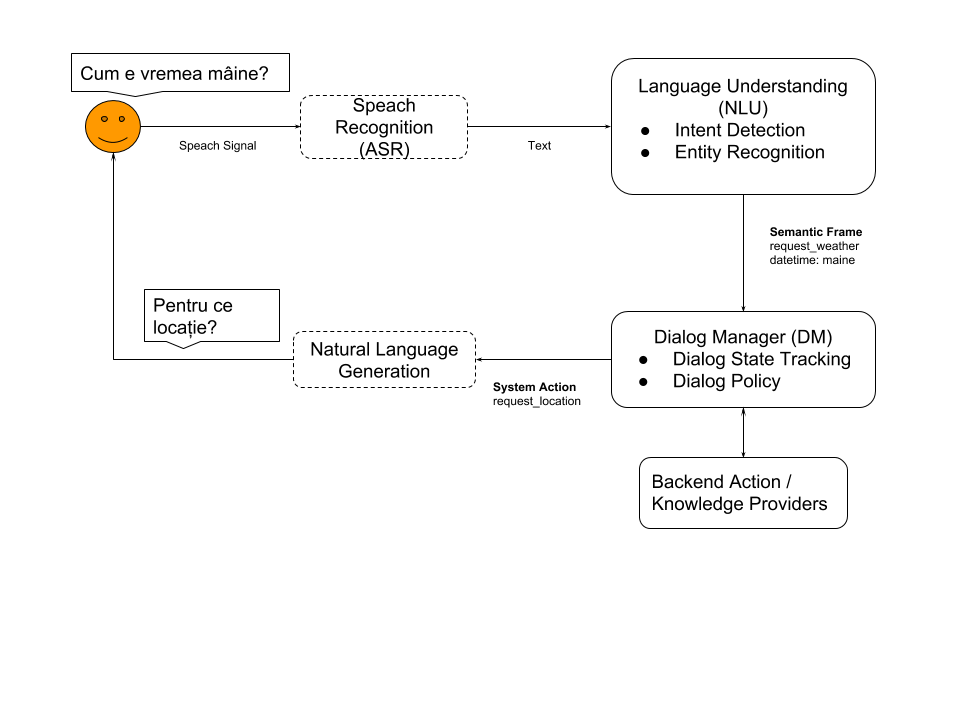
\includegraphics[scale=0.3]{dialog_system.png}
	\caption{Sistem de Dialog Modular}
	\label{fig:ds_proc}
\end{figure}
\begin{description}
	\item[Din voce în text - Speech To Text (STT)]  - 
	Este serviciul care se ocupă cu recunoașterea și conversia în text a semnalelor vocale
	\item[Înțelegerea limbajului natural - Natural Language Understanding (NLU)] -
	Componenta responsabilă de cadrul semantic ce descrie intenția și entitățile menționate de utilizator
	\item[Administrator de dialog - Dialog Manager (DM)] - 
	Este modulul ce gestionează dialogul, având ca funcții principale reprezentarea contextului și inferența pe baza acestuia
	\item[Generarea de limbaj natural - Natural Language Generation (NLG)] -
	Este modulul care se ocupă cu transformarea stării interne într-o replică de dialog
	\item[Din text în voce - Text To Speech] - 
	Ultima procesare este produsă de componenta care generează semnale vocale pe baza textului primit de la NLG
\end{description}

Întregul proces este descris de diagrama din figura \ref{fig:ds_proc}. Totul începe cu utilizatorul care formulează o cerere către sistem, vocea acestuia este procesată de către modulul de recunoaștere vocală care întoarce textul rostit de către vorbitor. Cererea în format text este apoi trimisă la modulul de înțelegere a limbajului care detectează la rându-i, intenția utilizatorului dar și entitățile menționate. Acest cadru semantic extras este apoi trimis modulului care ține firul dialogului și în funcție de definiția sarcinii pe care utilizatorul o dorește a fi îndeplinită se iau acțiunile în consecință și se trimite răspunsul către utilizator.

Doar componenta de înțelegere a limbajului și cea de administrare a dialogului vor fi analizate în cele ce urmează, întrunindu-se astfel minimul necesar unei conversații scrise.